\section{Optimisation problems}
Suppose we need to choose a rectangle with a fixed perimeter, but a maximal area. By considering the
symmetry of the problem, it is almost clear that if a solution exists then it \emph{should} be a square.

Indeed, suppose that our rectangle has side lengths $ x $ and $ y $, and perimeter $ \mathcal{P} $. Then $ \mathcal{P} = 2(x + y) $,
and so the area of our rectangle (the quantity we wish to maximise) is
\begin{displaymath}
  \mathcal{A} = xy = \frac{x(\mathcal{P} - 2x)}{2} = \frac{1}{2}\mathcal{P}x - x^2.
\end{displaymath}
Noting that the graph of the function $ \mathcal{A}(x) $ is a parabola, opening downwards, it is clear
that our desired maximum is the vertex; completing the square, we find that
\begin{displaymath}
  \mathcal{A} = \frac{1}{16}\mathcal{P}^2 - \left(x - \frac{1}{4}\mathcal{P}\right)^2
\end{displaymath}
and thus the vertex has $ x$--value $ \mathcal{P}/4 $; immediately, $ x = y $ and we see that our guess,
of a square optimal shape, was correct.

We were able to solve this problem because it ended up being equivalent to finding the maximum of a quadratic,
which is easy to solve in this way with only a little effort. However, consider the following problem, which is
essentially the same but now in three dimensions:
\begin{pro}
  Suppose a rectangular prism has two square faces of side length $ x $, and four rectangular faces with side lengths $ x $
  and $ y $; so the volume of the prism is $ x^2 y $. Let the perimeter $ \mathcal{P} = 8x + 4y $ of the prism be fixed.
  Find $ x $ and $ y $ satisfying this constraint such that the volume is maximised.
\end{pro}
Considering $ V = x^2y $, we substitute in our constraints:
\begin{displaymath}
  V = x^2 \left( \frac{\mathcal{P} - 8x}{4} \right) = \frac{\mathcal{P}}{2} x^2 - 2x^3
\end{displaymath}
and now we need to find the maximum value of a cubic --- which is not something we can do easily geometrically.

These types of problems are our motivation for the study in this section.

\begin{defn}
  If $ f $ is a function, then $ f $ is said to have a \emph{local maximum} at $ x_0 $ if there exists some (small)
  number $ \delta $ such that, for all $ x $ between $ x_0 - \delta $ and $ x_0 + \delta $, $ f(x) \leq f(x_0) $.

  Similarly, $ f $ is said to have a \emph{local minimum} at $ x_0 $ if there exists some number $ \delta $ such that,
  for all $ x $ between $ x_0 - \delta $ and $ x_0 + \delta $, $ f(x) \geq f(x_0) $.

  Local maxima and local minima are, collectively, called \emph{local extrema}. If we can take $ \delta $ as large
  as we like in either definition (e.g. if $ f(x) \geq f(x_0) $ for all possible $ x $ anywhere in the real numbers),
  we replace `local' with \emph{global}.

  For an illustration, see figure \ref{fig:localmin}.
\end{defn}

Many optimisation problems in applied mathematics can be reduced to finding relative extrema.

\begin{figure}
  \centering
  \begin{tikzpicture}
    \begin{axis}[
      axis lines = none,
      xlabel = $ x $,
      ylabel = {$ y = f(x) $}
    ]
      \addplot[domain = -3:3, color = black, samples = 100] {(1/6)*x^3 - (1/2)*x};
      \node[circle,fill,inner sep=2pt] at (axis cs:1,-1/3) {};
      \node[label={above:{$\left(x_0,f(x_0)\right)$}},circle,fill,inner sep=2pt] at (axis cs:1,-1/3) {};
      \draw[color=black!40, style=dotted] (0.15,-2) -- (0.15,2);
      \draw[color=black!40, style=dotted] (1.85,-2) -- (1.85,2);
      \node[label={below:{$x_0 - \delta$}}] at (axis cs:0.15,-2) {};
      \node[label={below:{$x_0 + \delta$}}] at (axis cs:1.85,-2) {};
    \end{axis}
  \end{tikzpicture}
  \caption{A local minimum of $ f $ at $ x_0 $ is a point lower than every other point in some interval around it.\label{fig:localmin}}
\end{figure}

\begin{exs}\leavevmode
  As in our first example above, many functions have local extrema that can be found with a little intelligent thought.
  \begin{enumerate}
    \item The function $ x \mapsto x^2 $ has a local minimum at $ (0, 0) $.
    \item The function $ x \mapsto 2x^3 + 15x^2 + 36x + 2 $ has a local maximum at $ (-3, -25) $ and a local minimum at $ (-2, -26) $.
    \item The function $ x \mapsto \sin x $ has a local maximum at $ (2n\pi + \frac{\pi}{2}, 1) $ for every integer $ n $, and
          a local minimum at $ (2n\pi - \frac{\pi}{2}, 1) $ for every integer $ n $.
  \end{enumerate}
\end{exs}

The main theorem is the following, which is a simple extension of the ideas from the last section on the geometry of the graphs
of functions. The basic geometric idea is that at a local extrema, the graph is changing from increasing to decreasing (or vice versa)
and thus the derivative is changing from a positive value to a negative value (or vice versa), and so must pass through zero.

\begin{thm}[Fermat]
  Let $ f $ be a function; suppose $ x_0 $ is a point in the interior of the domain of $ f $ (i.e. $ f(x) $ is defined for all $ x $ close
  to $ x_0 $ on both sides), that $ f $ is differentiable at $ x_0 $, and that $ f $ has a relative extremum  at $ x_0 $. Then $ f'(x_0) = 0 $.
\end{thm}
\begin{proof}
  Suppose $ x_0 $ is a local maximum of $ f $. Then for all $ x < x_0 $ such that $ x $ is `sufficiently close'\footnote{i.e. $ x $ lies
  within the $ \delta$-interval in the definition of a local maximum} to $ x_0 $, $ f(x) \leq f(x_0) $. Thus
  \begin{displaymath}
    \frac{f(x_0) - f(x)}{x_0 - x} \geq 0,
  \end{displaymath}
  since it is the quotient of two non-negative numbers.

  Similarly, for all $ x > x_0 $ sufficiently close to $ x_0 $, $ f(x) \leq f(x_0) $ and so
  \begin{displaymath}
    \frac{f(x_0) - f(x)}{x_0 - x} \leq 0.
  \end{displaymath}

  Since $ \lim_{x \to x_0} \frac{f(x_0) - f(x)}{x_0 - x} $ exists, the quantity $ \frac{f(x_0) - f(x)}{x_0 - x} $ must
  tend to the same value whether we approach from the left or from the right; and the only possible such value is zero.
\end{proof}

Motivated by this theorem, we define a \emph{critical point} of a function $ f $ to be some value $ x $ in the domain of $ f $ such
that either $ f'(x) = 0 $, or $ f'(x) $ is undefined. In the first case, we also call the value a \emph{stationary point}. All local
extrema occur at critical points, but not all critical points occur at extrema.

\begin{exs}\leavevmode
  \begin{enumerate}
    \item The function $ x \mapsto 2x^3 + 15x^2 + 36x + 2 $ above has critical points $ x = -2 $ and $ x = -3 $. Both of
          these are local extrema.
    \item The function $ x \mapsto x^3 $ above has a critical point at $ x = 0 $, but does not have a local extrema there.
    \item The function $ x \mapsto \frac{1}{x} $ \textbf{does not} have a critical point at $ x = 0 $, \textbf{because it is not defined there}.
  \end{enumerate}
\end{exs}

Utilising this technique, we can write down a recipe like the following to find extrema of a function $ f $ mechanically:
\begin{enumerate}
  \item Compute $ f' $.
  \item Find the points where $ f $ is defined but $ f' $ is not
  \item Find all the points where $ f' $ is zero.
  \item Find all the points $ x $ where $ f $ is defined at $ x $ and all points on one side of $ x $, but not the other.
  \item Then all the local extrema of $ f $ will be included in the lists of points in (2)--(3), and so we check each
        manually.
\end{enumerate}

There are two problems with this recipe. Firstly, the list of possible extrema may include points which are not actually
extrema and so we need a way to decide quickly whether a point is an extrema or a false alarm. This is something we will
address in a moment, so a more pressing concern is the second: finding zeroes of a function, in this case $ f' $, is just
as hard as finding extrema --- so we are only replacing one difficult problem with another.

\subsection{The geometry of critical points}
We can use the first derivative to classify extrema as either maxima or minima.
\begin{enumerate}
  \item Determine all critical points of $ f $.
  \item Determine the sign of $ f'(x) $ to the left and right of each critical point $ x_0 $:
    \begin{itemize}
      \item If $ f'(x) $ changes from positive to negative as we move from left to right across $ x_0 $, then $ f(x) $ has a local maximum at $ x_0 $.
      \item If $ f'(x) $ changes from negative to positive as we move from left to right across $ x_0 $, then $ f(x) $ has a local minimum at $ x_0 $.
      \item If $ f'(x) $ does not change sign across $ x_0 $, then $ f(x) $ does not have a relative extremum at $ x_0 $ (e.g. $ y = x^3 $).
    \end{itemize}
\end{enumerate}

On the other hand, using the second derivative, we can come up with a different test:
\begin{enumerate}
  \item Compute $ f'(x) $ and $ f''(x) $.
  \item Find all the stationary points of $ f $ by finding all the points $ x_0 $ such that $ f'(x_0) = 0 $.
  \item Determine the sign of $ f''(x) $ for each stationary point $ x_0 $:
    \begin{itemize}
      \item If $ f''(x_0) < 0 $ (i.e. $ f $ is concave down), then $ f(x) $ has a relative maximum at $ x_0 $.
      \item If $ f''(x_0) > 0 $ (i.e. $ f $ is concave up), then $ f(x) $ has a relative minimum at $ x_0 $.
      \item If $ f''(x_0) = 0 $ (i.e. $ f $ has an inflection point at $ x_0 $), then $ f(x) $ could have a relative maximum, a relative minimum, or neither.
    \end{itemize}
\end{enumerate}

\begin{ex}
  Find and classify the critical points of $ y = x^3 - 3x^2 + 6 $.

  \textit{Solution.} We have $ \od{y}{x} = 3x^2 - 6x $ and $ \od[2]{y}{x} = 6x - 6 $. Hence
                     the critical points are $ x = 0 $ and $ x = 2 $. At the former point, $ \od[2]{y}{x} < 0 $,
                     and so the point is a maximum; at the latter point, $ \od[2]{y}{x} > 0 $ and so the point is
                     a minimum.
\end{ex}

\begin{ex}
  Find two numbers whose difference is 100 and whose product is a minimum.

  \textit{Solution.} Let the two numbers be $ x $ and $ x + 100 $. We wish to minimise $ y = x(x + 100) $;
  clearly $ y' = 2x + 100 $, and so $ x = -50 $ is a critical point. To the left of $ x = -50 $, the derivative
  is negative; to the right, the derivative is positive. Hence $ x = -50 $ is indeed a minimum. The two required
  numbers are therefore -50 and 50.
\end{ex}

\begin{ex}
  Find and classify the critical points of $ y = (x - 1)^2 + \ln x $.

  \textit{Solution.} The derivative is $ y' = 2x - 2 + \frac{1}{x} $. We therefore have one critical
  point at $ x = 0 $ (where $ y' $ is undefined); this is an asymptote.
  Setting $ y' = 0 $, we have $ 0 = 2x - 2 + \frac{1}{x} = 2x^2 - 2x + 1 $ which has no real roots. Hence $ x = 0 $ is
  the only critical point, and the curve has no local extrema.
\end{ex}

\begin{ex}
  A rectangular plot of land is to be fenced using two varieties of fence. Two opposite sides will
  use fences selling for \$3 per metre, while the other two sides will use cheaper fence selling for \$2 per metre.
  Given that the total budget is \$1200, what is the greatest area of land which can be fenced?

  \textit{Solution.} Let $ x $ be the length of one of the expensive sides; then the length of one of the cheaper
                    sides is $ \frac{1}{2}(1200 - 3x) $, and the total area is $ A = \frac{1}{2} x (1200 - 3x) = \frac{1}{2}(1200x - 3x^2) $.
                    Hence $ \od{A}{x} = 600 - 3x $. We wish to find the maximum area, so set $ \od{A}{x} = 0 $; hence $ 3x = 600 $ and $ x = 200 $.
                    Note that the second derivative is always negative, so this stationary point must be a maximum as required. The length
                    of the other side will be $ \frac{1}{2}(1200 - 600) = 300 $, and so the maximum area is $ 300 \times 200 = 60000 $ square metres.
\end{ex}

\begin{ex}[Electric circuits]
  A battery of constant voltage $ \mathcal{E} $ and internal resistance $ \mathfrak{r} $ is connected to an external resistance $ R_\text{load} $.
  For what external resistance will the power $ P $ dissipated by the external resistance be maximal? (Possible application: we want to build a
  lamp to be connected to a particular voltage; what resistance should the filament be for maximum brightness?)

  \textit{Solution.} We have that $ P = I^2 R $, where $ I $ is the current through the circuit. Then $ I = \frac{\mathcal{E}}{\mathfrak{r} + R} $,
                     so $ P = \mathcal{E}^2 \frac{R}{(\mathfrak{r} + R)^2} $. In order to maximise this we will compute $ \od{P}{R} $:
                     \begin{displaymath}
                       \od{P}{R} = \mathcal{E}^2\frac{\mathfrak{r} - R}{(\mathfrak{r} + R)^3}, \qquad \od[2]{P}{R} = \mathcal{E}^2 \frac{3R - 3\mathfrak{r} - \mathfrak{r}R - R^2}{(\mathfrak{r} + R)^4}.
                     \end{displaymath}

                     Clearly $ \od{P}{R} = 0 $ precisely when $ R = \mathfrak{r} $; and in this case, $ \od[2]{P}{R} = \mathcal{E}^2(-2\mathfrak{r}^2)((2\mathfrak{r})^4) < 0 $, so this point is indeed a maximum for $ P $.

                     Thus the load should be given resistance equal to the internal resistance of the battery.
\end{ex}

\subsection{Exercises and Problems}
\begin{enumerate}
  \item Describe the advantages and disadvantages of the first and second derivative tests for local extrema.
  \item Describe the local extrema, concavity, and points of inflection of the function $ f(x) = x^4 - 4x^3 $.
  \item Consider the following graph:
        \begin{center}
          \begin{tikzpicture}[scale=.8]
            \begin{axis}[
              axis lines = center,
              xlabel = $ x $,
              ylabel = {$ y = f(x) $}
            ]
              \addplot[domain = -0.5:4, color = black, samples = 100] {x^3 - 4*x^2 + 3*x};
              \node[label={above:{$C$}},circle,fill,inner sep=2pt] at (axis cs:2.22,-2.11) {};
              \node[label={below:{$B$}},circle,fill,inner sep=2pt] at (axis cs:1.33,-0.74) {};
              \node[label={above:{$A$}},circle,fill,inner sep=2pt] at (axis cs:0.45,0.63) {};
            \end{axis}
          \end{tikzpicture}
        \end{center}
        Find the signs of $ \od{y}{x} $ and $ \od[2]{y}{x} $ at the three points $ A $, $ B $, and $ C $.
  \item Find all the local extrema of the following curves in the given intervals, and classify them as maxima, minima, or neither.
    \begin{enumerate}
      \item $ f(x) = \sin x - \cos x $ on the interval $ 0 < x < \pi $
      \item $ g(x) = x^3 - x^2 + x - 1 $ on the interval $ -\infty < x < \infty $
    \end{enumerate}
  \item The sum of two positive numbers $ x $ and $ y $ is 16. Find the smallest possible value for $ S = x^2 + y^2 $.
  \item A box with an open top is to be constructed from a square piece of cardboard with a side length of \SI{3}{\metre}
        by cutting out a square from each of the four corners and bending up the sides. Find the dimensions of the resultant
        box of maximum volume.
  \item Find the dimensions of a rectangle with area \SI{1000}{\metre\squared} such that the perimeter is minimised.
  \item A window consisting of a rectangle topped with a semicircle is to have a fixed perimeter $ p $. Find the radius
        of the semicircle in terms of $ p $ if the total area is to be maximised.
  \item A thin wire of length $ L $ is cut in two and the resulting lengths are bent to make a square and an equilateral triangle. Where
        should the wire be cut to make the total area of the shapes (a) a maximum and (b) a minimum?
  \item Find the point on the line $ y = 2x + 3 $ closest to the origin.
  \item Find the point on the curve $ y = \sqrt{x} $ closest to $ (3, 0) $.
  \item By finding the $ x$-- and $ y$-- intercepts, the asymptotes, the critical points, the
        intervals of increase and decrease, the intervals of concavity, and any other important
        points, sketch the following functions (199):
    \begin{enumerate}
      \item $ f(x) = \frac{x^2}{4 - x^2} $
      \item $ f(x) = \frac{4x}{x^2 + 1} $ [\textit{Hint: consider what happens to $ f(x) $ as $ x \to \pm\infty $.}]
      \item $ f(x) = \frac{x^2 - 4x + 5}{x - 2} = x - 2 + \frac{1}{x - 2} $ [\textit{Hint: consider what happens to $ f(x) - (x - 2) $ as $ x \to \pm\infty $.}]
    \end{enumerate}
  \item A cone with height $ h $ is inscribed in a larger cone of height $ H $ such that the vertex of the small cone
        is at the centre of the base of the larger cone. Show that the maximum volume of the smaller cone occurs when $ h = \frac{1}{3} H $.
  \item Show that the polynomial $ p(x) = 10x^3 + x^2 + x - 34 $ has exactly one real zero.
  \item A rain gutter is to be constructed from a metal sheet of width \SI{30}{\centi\metre} by bending up
        one third of the sheet on each side by an angle $ \theta $. What angle should be chosen in order to
        obtain the maximum possible volume?
  \item A steel pipe is carried around a right-angled corner from a hallway \SI{3}{\metre} wide into a hallway \SI{2}{\metre}
        wide. What is the length of the longest pipe that can be carried horizontally around the corner? [\textit{Hint: this is actually
        a minimisation problem, despite the wording.}]
  \item A large orange rectangle is to be drawn with one corner sitting on the origin and the opposite corner lying on
        the curve $ y = 0.2(x - 10)^2 $. What is the maximum possible area of the rectangle?
        \begin{center}
          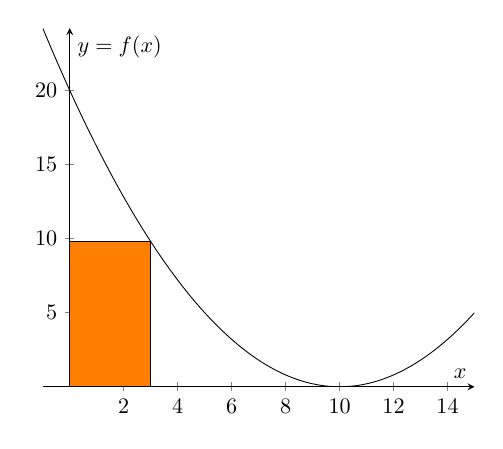
\begin{tikzpicture}[scale=.8]
            \begin{axis}[
              axis lines = center,
              xlabel = $ x $,
              ylabel = {$ y = f(x) $}
            ]
              \draw[fill = orange] (0,0) rectangle (3,9.8);
              \addplot[domain = -1:15, color = black, samples = 100] {0.2*(x - 10)^2};
            \end{axis}
          \end{tikzpicture}
        \end{center}
  \item Show that $ \frac{x^2 + 1}{x} \geq 2 $; hence (or otherwise) show that $ \frac{(x^2 + 1)(y^2 + 1)(z^2 + 1)}{xyz} \geq 8 $.
  \item Scholarship 2013: Prince Ruperts drops are made by dropping molten glass into cold water. A mathematical model for a drop
        as a volume of revolution uses $ y = \sqrt{\phi (e^{-x} - e^{-2x})} $ for $ x \geq 0 $, where $ \phi $ is the golden
        ratio $ \phi = \frac{1 + \sqrt{5}}{2} $.
    \begin{enumerate}
      \item Where is the modelled drop widest, and how wide is it there?
      \item The drop changes shape at a point $ B $, where the concavity of the function is zero. Use
            \begin{displaymath}
              \od[2]{y}{x} = \sqrt{\phi} \frac{e^{2x} - 6e^x + 4}{y^2 e^{4x}}
            \end{displaymath}
            to find the exact $ x$-ordinate of $ B $.
    \end{enumerate}
  \item Scholarship 2014: A family of functions is built from two functions $ f $ and $ g $, with a new function $ h_p $ defined
        for each value of $ p $, $ 0 \leq p \leq 1 $:
        \begin{gather*}
          f(x) = 2 + \sin x\\
          g(x) = 26 + \sin x\\
          h_p(x) = [f(x)]^{1 - p} [g(x)]^p.
        \end{gather*}
        Define a fourth function $ S $, where $ S(p) $ is the difference between the maximum and the minimum values of $ h_p $. Find
        the exact value of $ p $ that maximises $ S $.

        Note that if $ a $ is constant, $ \od{}{x} a^x = (\ln a) a^x $.
  \item Note that the second-derivative test may be inconclusive: if $ f'(x_0) = 0 $, and $ f''(x_0) = 0 $, then we may have
        an inflection point (like in the case of $ x \mapsto x^3 $), or a local extrema (like $ x \mapsto x^4 $). Looking at
        the second example here, one might conjecture that if we have a local extrema then $ f^{(n)}(x_0) > 0 $ for some large
        enough $ n $ (in the case of $ x^4 $, the fourth derivative is positive).

        Define $ f $ by
        \begin{displaymath}
          f(x) = \begin{cases} e^{-1/x^2} & x \neq 0 \\ 0 &x = 0 \end{cases}.
        \end{displaymath}
    \begin{enumerate}
      \item Show that $ f $ is differentiable at zero.
      \item Show that, for all $ n > 0 $, $ f^{(n)}(0) = 0 $. (Implicit here is the existence of the $ n$th derivative.)
      \item Show that $ f $ has a global minimum at zero.
      \item Justify that there can thus never be a rule, based simply on checking $ n$th derivatives, for proving
            that any function has a local minimum or maximum at a point. Hence our conjecture is false.
      \end{enumerate}
  \item Find $ x $, $ y $, and $ z $ positive real numbers such that the volume $ V = xyz $
        of the rectangular prism with these sidelengths is maximised, given that the perimeter
        of the prism is $ 4x + 4y + 4z = 12 $ and the surface area is $ 2xy + 2yz + 2zx = 6 $.
\end{enumerate}

\subsection{References}
For a significant number of optimisation exercises of the mechanical sort, see Stewart sections 4.1 and 4.7.

For more interesting problems, see Spivak chapter 11.

One avenue for further reading is the subject of the calculus of variations. See, for example, L\&S section 3.15,
as well as (for example) \emph{An introduction to the Calculus of Variations}, by Hans Sagan (Dover, 1992).

\subsection{Homework problems}
\begin{enumerate}
  \item What is the minimum vertical distance between the parabolae $ y = x^2 + 1 $ and $ y = x - x^2 $?
  \item Show that $ 3x + 2\cos x + 5 = 0 $ has exactly one real root by showing that it
        is increasing everywhere and crosses the $ x$-axis somewhere between two values of $ x $.
  \item Find the area of the largest rectangle that can be inscribed in the ellipse $ \frac{x^2}{a^2} + \frac{y^2}{b^2} = 1 $.
  \item Let $ ABCD $ be a square piece of paper with sides of length \SI{1}{\metre}. A
        quarter-circle is drawn from $ B $ to $ D $ with centre $ A $. The piece of paper is folded along $ EF $, with $ E $ on $ AB $
        and $ F $ on $ AD $, so that $ A $ falls on the quarter-circle. Determine the maximum and minimum areas that the triangle $ AEF $
        can have. [\textit{Hint: you may want to introduce a coordinate system.}]
\end{enumerate}
